\section{Computer Vision}
On top of the various training and learning algorithms, another cornerstone of fully autonomous robot movement is computer vision. Through the integration of visual sensors (and possibly others to support and reinforce robot perception) and advanced image processing techniques, robots can be taught to identify surroundings and make informed decisions. 

Although autonomisation is possible without vision, having a generalisable view of an environment or task allows a robot to be a generic executor. Take for example a factory robot assembling cars. It can be efficiently made automatic without any complicated models, and with just a simple algorithm. However this means that the environment (i.e the car parts, and maybe the work-area layout) must be presented in identical configurations for each episodic repetition of the task.
As the focus in robotics is shifting towards generic and dynamically moving robots which need to adapt to their environments, vision becomes an inevitable sensing medium.

\subsection{The Camera Model}
Camera models are essential for vision. As us humans perceive the world in an analogue manner through light, the robot must also be able to interpret its surroundings the same way. A \emph{camera} is a device that captures light in a scene and a \emph{camera model} is therefore defined to be the how that analogue information is mapped onto a 2D coordinates in a mathematical manner \cite{zhang2021cameramodels}. 

An essential process when using a camera is calibration. This is required so that we can normalise what the robot ``sees'' and using some pre-defined criteria (such as a known object or a pattern) so that we can be assured the information the camera provides is within a specified degree of confidence. This uncertainty range should be as low as possible as tasks like localisation, mapping and object interactions in robotics usually require precise camera measurements.

While calibrating we need to have some idea of physical properties of the camera (\emph{intrinsic}) and information about the mappings of the scene (\emph{extrinsic}).

\subsubsection{Intrinsic Parameters}\label{sec:intrinsic}
These cover the internal characteristics of the camera, and how the captured three dimensional (3D) world data will be projected down onto the two dimensional (2D) image plane. Some important parameters are:

\begin{itemize}
  \item \textbf{Focal Length ($f$):} The distance netween the camera lens and the image sensor. Determines field of view (FOV) and required for scaling the scene.
  \item \textbf{Principal Point (c):} Point of intersection for the optical axis and image plane. Usually at the centre of the image.
  \item \textbf{Skew (s):} Non-orthogonality factor of the sensor axes of the camera. (Often zero in most camera models as most modern cameras have no significant shearing in the image they create)
  \item \textbf{Distortion Coefficients:} Some parameters for distortion correction. Important for camera model systems like cameras with fish-eye lenses \cite{king1989history}
\end{itemize}

\subsubsection{Extrinsic Parameters}
Extrinsic parameters represent the physical placement of the camera in the scenes. Such as the position and orientation of the camera in the scene. Using these values we can map  3D representation of the world the camera sees (which is in world coordinates) into the camera coordinate system. The mapping of parameters to the camera view is shown in Figure \ref{fig:in-extrinsic}.

\begin{figure}[h]
  \centering
  \begin{subfigure}{0.45\linewidth}
    \centering
    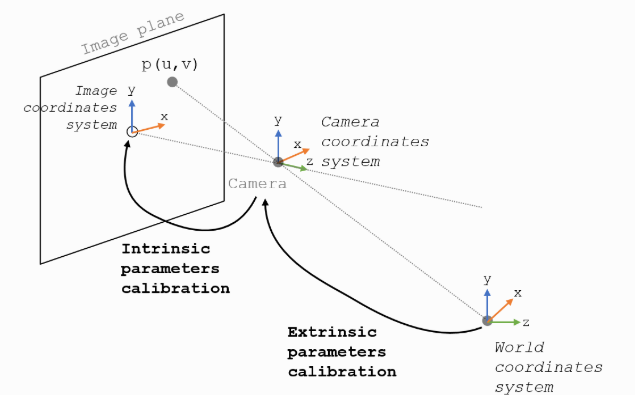
\includegraphics[width=\linewidth]{assets/background/in-extrinsic.png}
    \caption{Intrinsic and extrinsic parameter mappings \cite{mphy0026camera}}\label{fig:in-extrinsic}
  \end{subfigure}
  \hfill
  \begin{subfigure}{0.45\linewidth}
    \centering
    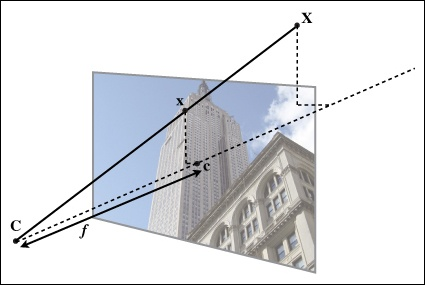
\includegraphics[width=\linewidth]{assets/background/pinhole-cam.jpg}
    \caption{Pinhole camera model \cite{solem2012programming}}\label{fig:pinhole}
  \end{subfigure}
  \caption{Camera Models}\label{fig:cam-models}
\end{figure}

\subsection {The Pin-Hole Camera}
One of the most foundational and widely used models to describe this calibration is the \emph{pin-hole} (or the  \emph{projective}) camera model \cite{solem2012programming}. 

\subsubsection{Mathematics Behind the Pin-Hole Model}
The light passes through a single point, called the camera centre, $C$, before it is projected onto the 2D image plane (giving the name pin-hole). A 3D point $\textbf{X}$ is projected onto image point $\textbf{x}$ using the equation:
\(\lambda \textbf{x} = P\textbf{X}\). where $P$ is the a 3x4 matrix called the camera (or \emph{projection}) matrix and $\textbf{X}$ is 1x4 and has four elements in homogenous coordinates, \(\textbf{X} = [x, y, z, w]\) and $\lambda$ is the inverse depth of the 3D point. Which can be needed if we want all coordinates to be homogenous with the last value ($w$) normalised to $1$.
The Camera Matrix, P can will all calibration values for the camera. So: \(P = K \left[R \mid t\right] \), $R$ is the ($3 \times 3$) rotational matrix describing the orientation of the camera, and t a ($3 \times 1$) translational vector describing the position of C.Also the intrinsic calibration matrix, K, will encode camera attributes discussed above.
\[
  K = 
  \begin{bmatrix}
    f_x & s & c_x \\
    0 & f_y & c_y \\
    0 & 0 & 1
  \end{bmatrix}
  \hspace{1cm}
  f_x = \alpha f_y
\]

Where the values are from \ref{sec:intrinsic} and $\alpha$ is the aspect ratio used for non-square pixel elements (usually safe to assume $a=1$). A simple calibration method is to use a reference object, with known dimensions $dX and dY$. Then we can measure the distance from the camera to the object $dZ$. After obtaining the image we can measure the image plane size of our object $dx, dy$ in pixels and extract the focal point as: \(
  f_x = \frac{dx}{dX} dZ , \hspace{1cm} f_y = \frac{dy}{dY}dZ
  \)Or we can use a calibration image to project and use that for calibration, see Figure \ref{fig:calin-dots}

  \begin{figure}[h]
    \centering
    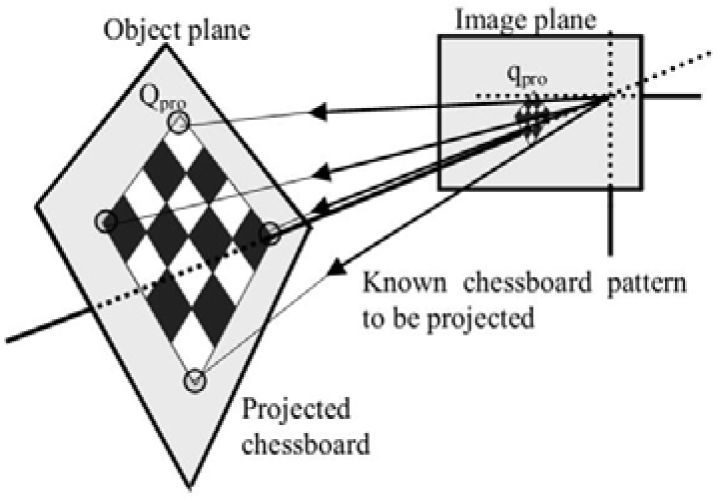
\includegraphics[width=0.4\textwidth]{assets/background/checkered.jpeg}
    \caption{Calibration pattern cite{Din2014ProjectorCalibration}}\label{fig:calin-dots}
  \end{figure}

\subsection{Other Camera Models for Robotics}
The pin-hole camera system gives us an insight into the translation of captured light into interpretable data. Although, useful for theoretical analysis, real-world cameras deviate from this idealised system quite a lot.
There are different lens models like the \emph{thin-lens} model which -opposing the pin-hole model- doesn't assume an infinitely small aperture. Mimicking the real world closer as cameras need lenses to focus the light. And these lenses add to the intrinsic properties of the camera.

\subsubsection{Different Fields of View (FOV)}
Cameras providing different FOVs such as fish-eye or wide-angle cameras, for different degrees of vision. For example, 360-degree cameras for surveillance or autonomous driving. Where the distortion of the image must be corrected in processing.

\subsubsection{Multiple Cameras}
\emph{Stereo camera models} (Binocular vision) for depth measurement incorporation into the image. Two cameras which are a known distance apart can be used to perceive depth by computing the disparity between corresponding points in both images (triangulation) \cite{hamzah2016literature}. This can also be scaled to \emph{n-view stereo vision} to reduce occlusion problems while increasing redundancy in the number of viewpoints there are.\label{sec:nview}

\subsubsection{Active Depth Cameras}
These go beyond stereo vision. Such as \emph{Time-of-Flight (ToF)} cameras that emit infra-red light and measure the time it takes to reflect back, and using speed of light in calculating the depth directly \cite{foix2011tof,zanuttigh2016time}. Or \emph{structured light} cameras that project a known pattern onto a surface and observe its deformation to calculate the depth. These two are usually more concise compared to stereo vision because they offer robust depth sensing regardless of surface textures or differing lighting conditions.
\\\\
Therefore, choice of camera model significantly affects how a robot can perceive its environment and its calibration impacts the degree of correctness.

\subsection{Visual Perception and Object Recognition}
  The goal of computer vision within robotics is to alow the robot to infer meaningful information about its surroundings and later use that information to achieve its goals. So, perception starts with understanding what is in the scene to a macro and micro level. 
  
  \subsubsection{Low-Level Vision}
    These are fundamental visual features without caring about the details of what the overlying object may be. Such as: detecting colours, corners, edges of objects. 

  \subsubsection{High-Level Vision}
    This, on the other hand, is where the learnt small information can be transformed up to generalise into tasks such as object recognition, motion tracking and most importantly scene interpretation.
    \\\\
    Traditional Computer Vision approaches relied on manually crafted systems to extract features from images:
    \begin{itemize}
      \item \textbf{Edge Detection:} Identifying mathematically distinct features such as edges and corners \cite{marr1980theory} which can then be used for object recognition. Using methods such as Canny Edge detection \cite{canny1986computational} and Harris Corner Detector \cite{derpanis2004harris}.
      \item \textbf{Feature Descriptors:} Extracting keypoints and descriptors from images, allowing for object matching across different scales and orientations. Utilising methods like SIFT (Scale-Invariant Feature Transform), SURF (Speeded-Up Robust Features) \cite{wu2013comparative,juan2009comparison} and ORB (Oriented FAST and Rotated BRIEF) \cite{rublee2011orb}.
      \item \textbf{Template Matching:} Compares an input image to stored reference images to detect images that are in the known objects database. Usually useful when the environment can be controlled \cite{brunelli2009template}.
    \end{itemize}

    However successful these methods have been in structured settings, they don't necessarily do well with large variations in object appearance, real-world noise and dynamic backgrounds. Therefore, these can't necessarily be easily extended to work in a dynamic robotics setting.

    \subsubsection{Deep Learning-Based Approaches}
    Modern object detection and recognition is mostly reliant on deep learning methods:
    \begin{itemize}
      \item \textbf{Convolutional Neural Networks (CNNs):} These \cite{gu2018recent,li2021survey} can automatically learn hierarchical features from raw image data. Which can then be used for image classification \cite{hijazi2015using,traore2018deep}, while being robust to variations in lighting, occlusions, and perspective changes.
      \item \textbf{Region-Based CNNs (R-CNN):} These models propose candidate regions and run CNNs on that region for classifying with higher accuracy in complex scenes \cite{bharati2020deep, girshick2015fastrcnn}
      \item \textbf{Transformer Architectures (ViTs):} Recent advances in transformer architectures \cite{bi2021transformer} now being used in vision using attention mechanisms to improve object detection in cluttered environments \cite{kayacan2024vision} and be robust against long-range dependencies which CNN's suffer from due to locality of processing.
    \end{itemize}

  \subsection{Applying to Robotics}
    Despite these significant advances within Computer Vision, there are still some challenges that are present within vision in robotics that must be addressed in making a human-like dynamically learning and moving robot.

    \subsubsection{Lighting and Appearance}
      Due to expectations of robots being dynamic, they must be able to operate in varying environments where lighting and scene appearances will be constantly changes.

    \subsubsection{Occlusions}
      Within real life dynamic environments, on top of the lighting changes, object are often partially or sometimes fully occluded from where the robot might be placed or moving in the environment.  One of the simple solutions to this is to introduce multiple views for the robot. 
      
      Similar in idea to \emph{n-view} from \ref{sec:nview}, having more cameras, usually some around the scene and some on different parts of a robot (e.g. wrist-mounted, head-mounted, or mounted around the scene) allows for robustness against occlusions and introduce multiple different angles for efficiency in learning. 

      However, one big drawback is that the state space can easily explode: increasing training times and inferring speeds. On top of that, depending on the task and the robot multi-viewpoint systems might not be feasible, for example, the environment might not be as clearly defined, making the such cameras an impossibility. There are other solutions such as temporal consistency \cite{lai2018learningblindvideotemporal} which can also be extended for use in robotics, such as here \cite{billington2007using, yang2021reactive}.
      \todo[color=green]{maybe some figures here from tasks like searching drawer etc.}

      \begin{figure}[h]
        \centering
        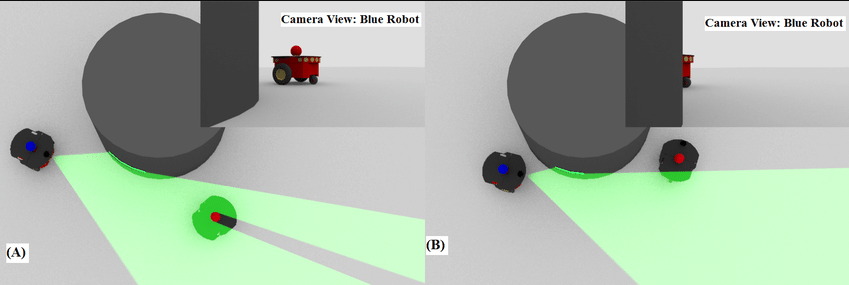
\includegraphics[width=0.7\textwidth]{assets/background/occlusion.png}
        \caption{Example of an occluded object \cite{occlusionimage}}\label{fig:occlusion}
      \end{figure}
      \todo[color=green]{better image}

    \subsubsection{Real-Time Processing}
    Another convoluted problem in vision to robotics is that, novel advancements are usually resource intensive and then scaled down once proven. Many autonomous real-time  applications such as autonomous driving, drone navigation need provably quick decision making in order to be safe to use. Therefore computational bottlenecks or unoptimised approaches requiring time and computational resources might not immediately fit into a robotics use case.

    \subsubsection{Unseen Domain Generalisations}
    Finally, another active area in robotics currently is issues such as \emph{few-shot} or even \emph{one-shot} learning see \ref{sec:few-shot}, which aim to teach robots new and unseen policies with minimal new data. Or approaches such as self-supervised learning (such as here \cite{lim2022real2sim2real, huang2021robot}) to combine real and simulated data for optimising learning in new domains.
    \\\\
    One of the trajectories that can be taken in improving such static models is to take inspiration from what makes humans good visual learners. We also face issues like occlusions in day-to-day life and one advantage we have is that our vision is \textbf{active.}
    
  

    